\question[10] La Tabla \ref{tab:recorrido_auto} muestra la distancia que un automóvil recorre en el tiempo indicado.

\begin{minipage}{.6\textwidth}
    \begin{table}[H]
        \centering
        \caption{Datos sobre el recorrido de un automóvil}
        \label{tab:recorrido_auto}
        \begin{tabular}{c|c|c|c|c}
            Distancia (km) & 20             & 60              & 80 & 100             \\
            \hline
            Tiempo (h)     & $\dfrac{1}{2}$ & 1$\dfrac{1}{2}$ & 2  & 2$\dfrac{1}{2}$ \\
            \bottomrule
        \end{tabular}
    \end{table}

    \begin{parts}
        \part  Si el automóvil pasa por el kilómetro cero y se mueve siempre con la misma
        velocidad, ¿qué distancia recorrerá en 4 horas?
        \part  ¿La relación entre las variables corresponde a una relación de variación proporcional? ¿Por qué?
        \part  Grafica en el plano cartesiano de la Figura \ref{fig:recorrido_auto} los puntos que indican
        los datos de la Tabla \ref{tab:recorrido_auto} y únelos con una línea.
        \part Redacta una manera de obtener, a partir de la gráfica de la Figura \ref{fig:recorrido_auto}, la distancia que el
        automóvil recorre en un tiempo dado.
    \end{parts}

\end{minipage}\hfill
\begin{minipage}{.25\textwidth}
    \begin{figure}[H]
        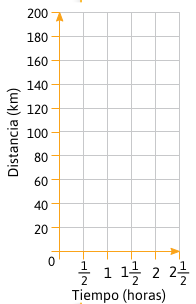
\includegraphics[width=0.9\linewidth]{../images/recorrido_auto_blank.png}
        \caption{Gráfica del recorrido de un automóvil.}
        \label{fig:recorrido_auto}
    \end{figure}
\end{minipage}


